%%%%%%%%%%%%%%%%%%%%%%%%%%%%%%%%%%%%%%%%%%%%%%%%%%%%
%
% Adapted to English and filled with thesis content
% for the University of Trieste theme by Isac Pasianotto.
%
%%%%%%%%%%%%%%%%%%%%%%%%%%%%%%%%%%%%%%%%%%%%%%%%%%%%

\documentclass{beamer}

% Load all required packages for the theme
\usepackage{otherResources/presentazione_allPackages}
\usetikzlibrary{shapes.geometric, positioning}
\usetikzlibrary{shapes.arrows, positioning}
\usetikzlibrary{positioning,calc,arrows.meta,fit,backgrounds,matrix}

% Document metadata
\hypersetup{
	pdfauthor={Nicola Perin},
	pdftitle={Designing and deploying a FAIR-by-design data pipeline and platform for electron microscopy laboratories},
	pdfsubject={Research thesis in: Data Management}
}

% Title block
\title[FAIR-by-design EM pipeline]{Designing and deploying a FAIR-by-design data pipeline and platform for electron microscopy laboratories}
\subtitle{Research thesis in: Data Management}
\institute{University of Trieste}
\author[Nicola Perin]{Nicola Perin}
\year=2025
\month=09
\day=19

% Advisors & labels (translated to English)
\def\relatore{Dott. Federica Bazzocchi}
\def\relatoreLabel{Supervisor}
% \def\correlatore{<Co-supervisor name>}
% \def\correlatoreLabel{Co-supervisor}
\def\candidatoLabel{Candidate}

% Logos (use your local paths if different)
\def\LogoUniversita{otherResources/Units.Logo3Righe.png}
\def\LogoDipartimento{otherResources/DSSC_logo.png}
\def\LogoFiligrana{otherResources/background-blu.png}

% Apply theme customizations
%%%%%%%%%%%%%%%%%%%%%%%%%%%%%%%%%%%%%%%%%%%%%%%%%%%%%%%%%%%
%
% Copyright 2022 by Isac Pasianotto
%
% This file may be distributed and/or modified
%
% 1. under the LaTeX Project Public License and/or
% 2. under the GNU Public License.
%
%%%%%%%%%%%%%%%%%%%%%%%%%%%%%%%%%%%%%%%%%%%%%%%%%%%%%%%%%%%

%% 	Variabili di tipo "color": 

\definecolor{bluUnits100}{rgb}{0.16,0.22,0.36} 
\definecolor{bluUnits80}{rgb}{0.22,0.3,0.51}
\definecolor{bluUnits70}{rgb}{0.25,0.35,0.58}
\definecolor{bluUnits50}{rgb}{0.41,0.51,0.74}
\definecolor{bluUnits40}{rgb}{0.56,0.63,0.81}
\definecolor{bluUnits25}{rgb}{0.78,0.82,0.9}
\definecolor{bluUnits10}{rgb}{0.93,0.94,0.96}
\definecolor{grey}{rgb}{0.3686, 0.5255, 0.6235} 

%%	Palette di colori 

\setbeamercolor{palette primary}{bg=bluUnits100,fg=white}
\setbeamercolor{palette secondary}{bg=bluUnits80,fg=bluUnits25}
\setbeamercolor{palette tertiary}{bg=bluUnits50,fg=bluUnits100}
\setbeamercolor{palette quaternary}{bg=bluUnits40,fg=white}
\setbeamercolor{palette light primary}{bg=bluUnits25,fg=bluUnits100}
\setbeamercolor{palette titleframe}{bg=bluUnits10, fg=bluUnits80}


		%%%%%%%%%%%%%%%%%%%%%%%%%%%%%%%%%%
		%% Impostazioni generali slide  %%
		%%%%%%%%%%%%%%%%%%%%%%%%%%%%%%%%%%

%%	Setta l'immagine da mettere come sfondo, riducendone l'opacità
\usebackgroundtemplate{\tikz\node[opacity=0.1]{\includegraphics[height=\textheight]{\LogoFiligrana}};}

%%	Elenchi puntati, numerati, etc.

\setbeamercolor{structure}{fg=bluUnits80}
\setbeamertemplate{enumerate item}[circle]
\setbeamertemplate{itemize subitem}[ball]
% Valutare a secoda del contesto se sostituire con 
% \setbeamertemplate{items}[circle]
\setbeamercolor{alerted text}{fg=bluUnits50}

%% 	Colore delle scritte nella presentazione

\setbeamercolor{normal text}{fg=bluUnits100,bg=white}

%% 	Settaggio della linea in alto (headline)

\setbeamertemplate{headline}{
	\vskip1pt
	\leavevmode	
	\hbox{
		\begin{beamercolorbox}[wd=.99\paperwidth,ht=2.5ex,dp=1.125ex]{palette light primary}
			\insertsectionnavigationhorizontal{\paperwidth}{}{\hskip0pt plus1filll}
		\end{beamercolorbox}
	}
}

%%	Settaggio riga in basso (footline) 
 
\setbeamertemplate{footline}{
       \leavevmode
	   \hbox{
           \begin{beamercolorbox}[wd=.2\textwidth,ht=2.6ex,dp=1ex,center]{palette tertiary}
		    \usebeamerfont{author in head/foot}\insertshortauthor
    	\end{beamercolorbox}
	
    	\begin{beamercolorbox}[wd=.27\textwidth,ht=2.6ex,dp=1ex,center]{palette quaternary}
	   		\usebeamerfont{institute in head/foot}\insertshortinstitute
	   	\end{beamercolorbox}
	
    	\begin{beamercolorbox}[wd=.40\textwidth,ht=2.6ex,dp=1ex,center]{palette primary}
    		\usebeamerfont{title in head/foot}\insertshorttitle
    	\end{beamercolorbox}

    	\begin{beamercolorbox}[wd=.1\textwidth,ht=2.6ex,dp=1ex,center]{palette light primary}
	   		\insertframenumber{}/\inserttotalframenumber
	    \end{beamercolorbox}
    }
    \vskip2pt

}

%%	Settaggio tittoli delle slide  

\setbeamertemplate{frametitle}{
	\begin{beamercolorbox}[wd=\paperwidth,ht=2.75ex,dp=1ex,left]{palette titleframe}
		\qquad \textbf{\insertframetitle}
	\end{beamercolorbox}
}


		%%%%%%%%%%%%%%%%%%%%%%%%%%%%%%%
		%% Impostazioni Prima Slide  %%
		%%%%%%%%%%%%%%%%%%%%%%%%%%%%%%%
	
	
	
	
		
\def\setTitlestyleDissertation{
	
	\defbeamertemplate*{title page}{customized}[1][]{
		
		%  Commentare il seguente ambiente {center} e decommentare {flushright} quello successivo in caso
		%	si voglia usare solo il logo dell'UNI
		
		\begin{center}
			\begin{multicols}{2}
				\includegraphics[width=0.45\textwidth]{\LogoDipartimento}
			\columnbreak
				\includegraphics[width=0.45\textwidth]{\LogoUniversita}		
			\end{multicols}
		\end{center}
	
		%	\begin{flushright}
		%		\includegraphics[width=0.45\textwidth]{\LogoUniversita}	
		%	\end{flushright}
	
		\smallskip
		
		\begin{center}		
			\usebeamerfont{title}\textbf{\inserttitle}\par
			\usebeamerfont{subtitle}\usebeamercolor[fg]{subtitle}\insertsubtitle\par
			\medskip		
			
			%% Il seguente layout dentro l'ambiente multicols serve per le tesi.
			
			\begin{multicols}{2}
				\begin{tabular}{c}
					\usebeamerfont{normal text}{\relatoreLabel} \\
					\usebeamerfont{author}{\relatore}
					
						% Decommentare in caso siano presenti dei correlatori
					%\\
					%\usebeamerfont{normal text}{\correlatoreLabel} \\
					%\usebeamerfont{author}{\correlatore}
						
				\end{tabular}					
				\columnbreak
				\begin{tabular}{c}
					\candidatoLabel \\
					\usebeamerfont{author}{\insertauthor}
				\end{tabular}
			\end{multicols}
		
			\par
			
			\bigskip  	% --> nel caso di relatore e basta
			%\smallskip 	% --> nel caso di relatore + correlatore
			
			\insertinstitute\par
			
			\bigskip	% --> nel caso di relatore e basta
			%\smallskip	% --> nel caso di relatore + correlatore
			
			\usebeamerfont{date}\insertdate\par
			
			\bigskip	% --> nel caso di relatore e basta
			%\smallskip	% --> nel caso di relatore + correlatore
		\end{center}
	}
}


% ---- Slides ----
\begin{document}
	
	% =====================
	% Title & Agenda
	% =====================
	
	% Title frame (special dissertation style from the theme)
	\begin{frame}
		\setTitlestyleDissertation
		\maketitle
	\end{frame}
	
	% --- Outline ---
	\begin{frame}
		\frametitle{Outline}
		\begin{enumerate}
			\item Electron microscopy data: what it looks like and where the problems are
			\item FAIR principles and the NeXus (NXem) standard
			\item The case study: LAME and the ORFEO datacenter
			\item From lab problems to a proposal
			\item Designing the web application
			\item Testing with VirtualOrfeo
			\item Walking through the app
			\item Live demo
		\end{enumerate}
	\end{frame}
	
	% =====================
	% Story: Intro → FAIR → Case Study → Design → VirtualOrfeo → App Walkthrough
	% =====================
	
	% --- 1) Intro: EM, data, issues, needs ---
	
	\begin{frame}
		\frametitle{Electron microscopy data: an overview}
		
		\begin{itemize}
			\item Instruments (TEM, SEM, STEM) generate images, diffraction patterns, and spectra —
			often multi-terabyte datasets.
			\item Each vendor uses their own file formats; metadata is often incomplete or inconsistent.
			\item Day-to-day handling is messy: manual copies, endless zip files, unclear provenance.
			\item This makes collaboration and reuse difficult.
		\end{itemize}
		
		\vspace{0.5em}
		\small\textit{The challenge: how do we handle this data so it remains usable and shareable?}
	\end{frame}
	
	% --- FAIR + NeXus (rewritten) ---
	\begin{frame}
		\frametitle{A way forward: FAIR and NeXus (NXem)}
		\begin{columns}[T,totalwidth=\textwidth]
			\column{0.55\textwidth}
			\begin{itemize}
				\item FAIR principles: \textbf{findable, accessible, interoperable, reusable}.
				\item \textbf{HDF5}: efficient format for large, structured datasets.
				\item \textbf{NeXus}: conventions for scientific data (\texttt{NXinstrument}, \texttt{NXsample}).
				\item \textbf{NXem}: application definition tailored to electron microscopy.
			\end{itemize}
			\column{0.45\textwidth}
			
\includegraphics[width=\textwidth]{otherResources/FAIR_data_principles.png}
			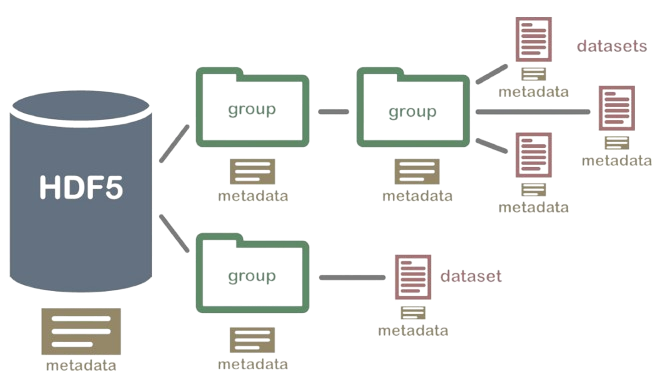
\includegraphics[width=\textwidth]{otherResources/HDF5_diagram.png}
			
\includegraphics[width=\textwidth]{otherResources/NEXUS_logo.png}
		\end{columns}
		\vspace{0.5em}
		\small At the national level, these FAIR practices are promoted and supported by the NFFA-DI infrastructure.
	\end{frame}
	
	% --- NFFA-DI introduction (new slide) ---
	\begin{frame}
		\frametitle{Introducing NFFA-DI}
		\begin{columns}[T,totalwidth=\textwidth]
			\column{0.55\textwidth}
			\begin{itemize}
				\item \textbf{NFFA-DI} = Nano Foundries and Fine Analysis – Digital Infrastructure.
				\item Italian research initiative connecting major nanoscience centers.
				\item Goal: open access to advanced instrumentation, FAIR data, and computational resources.
				\item Acts as the national driver for FAIR data practices in nanoscience.
			\end{itemize}
			\column{0.5\textwidth}
			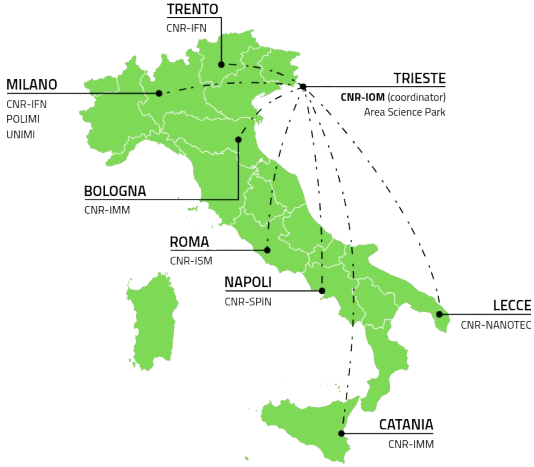
\includegraphics[width=\textwidth]{otherResources/NFFA_map.png} % replace with your map image
			\vspace{2em}
			\tiny Source: \url{https://nffa-di.it/en/}
		\end{columns}
	\end{frame}
	
	% --- Introducing LAME ---
	\begin{frame}
		\frametitle{Introducing LAME}
		
		\begin{itemize}
			\item LAME = Electron Microscopy Lab at Area Science Park, opened in 2022.
			\item Core instrument: a \textbf{double-corrected TEM/STEM} with advanced detectors.
			\item Enables atomic-scale imaging, spectroscopy, and in situ experiments 
			(gas, heating, electrical bias).
			\item Supports nanoscience projects within NFFA-DI and European collaborations.
		\end{itemize}
	\end{frame}
	
	% --- 2) Case study: LAME @ Area Science Park, ORFEO storage, current gap ---
	\begin{frame}
		\frametitle{From the lab to the datacenter}
		
		\begin{columns}[T,totalwidth=\textwidth]
			% Left column: text
			\column{0.55\textwidth}
			\begin{itemize}
				\item \textbf{LAME} produces multi-terabyte datasets in electron microscopy.
				\item As part of NFFA-DI, its work depends on sharing data with other partners.
				\item To support this, \textbf{ORFEO} provides the backbone: HPC resources, 
				identity services, and S3-compatible object storage.
				\item The challenge: connecting LAME’s lab workflows with ORFEO’s infrastructure.
			\end{itemize}
			
			% Right column: stacked images + arrow
			\column{0.45\textwidth}
			\centering
			\begin{tikzpicture}[node distance=1.0cm]
				% microscope node
				\node (microscope) at (0,0.5) {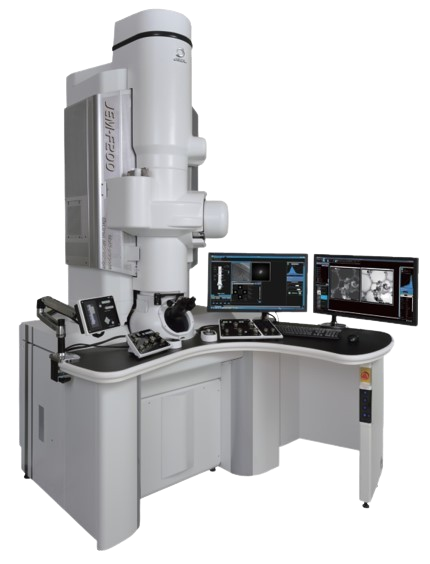
\includegraphics[width=0.5\textwidth]{otherResources/LAME_microscope.png}};
				% orfeo node placed below with manual shift
				\node (orfeo) at (0,-3.0) {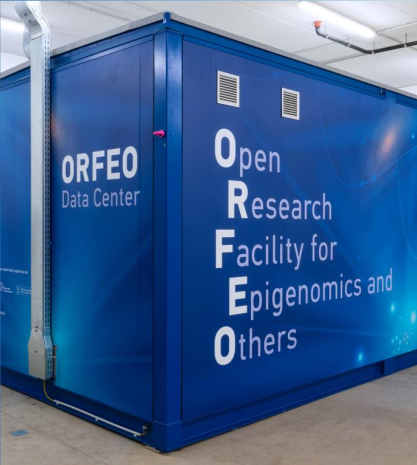
\includegraphics[width=0.5\textwidth]{otherResources/ORFEO.png}};
				% arrow
				\draw[->, line width=1.5mm, blue!60!black] ([yshift=+5mm]microscope.south) -- (orfeo.north);
			\end{tikzpicture}
		\end{columns}
	\end{frame}
	
	\begin{frame}
		\frametitle{ORFEO’s storage model}
		
		For LAME, ORFEO relies on an \textbf{object storage} system:
		
		\begin{itemize}
			\item An \textbf{object} is a file together with all the metadata that describes it.
			\item A \textbf{bucket} is a container that holds objects (like a project folder, but flatter).
			\item Access is through the \textbf{S3 protocol}, which is scalable and widely supported.
		\end{itemize}
		
		\centering
		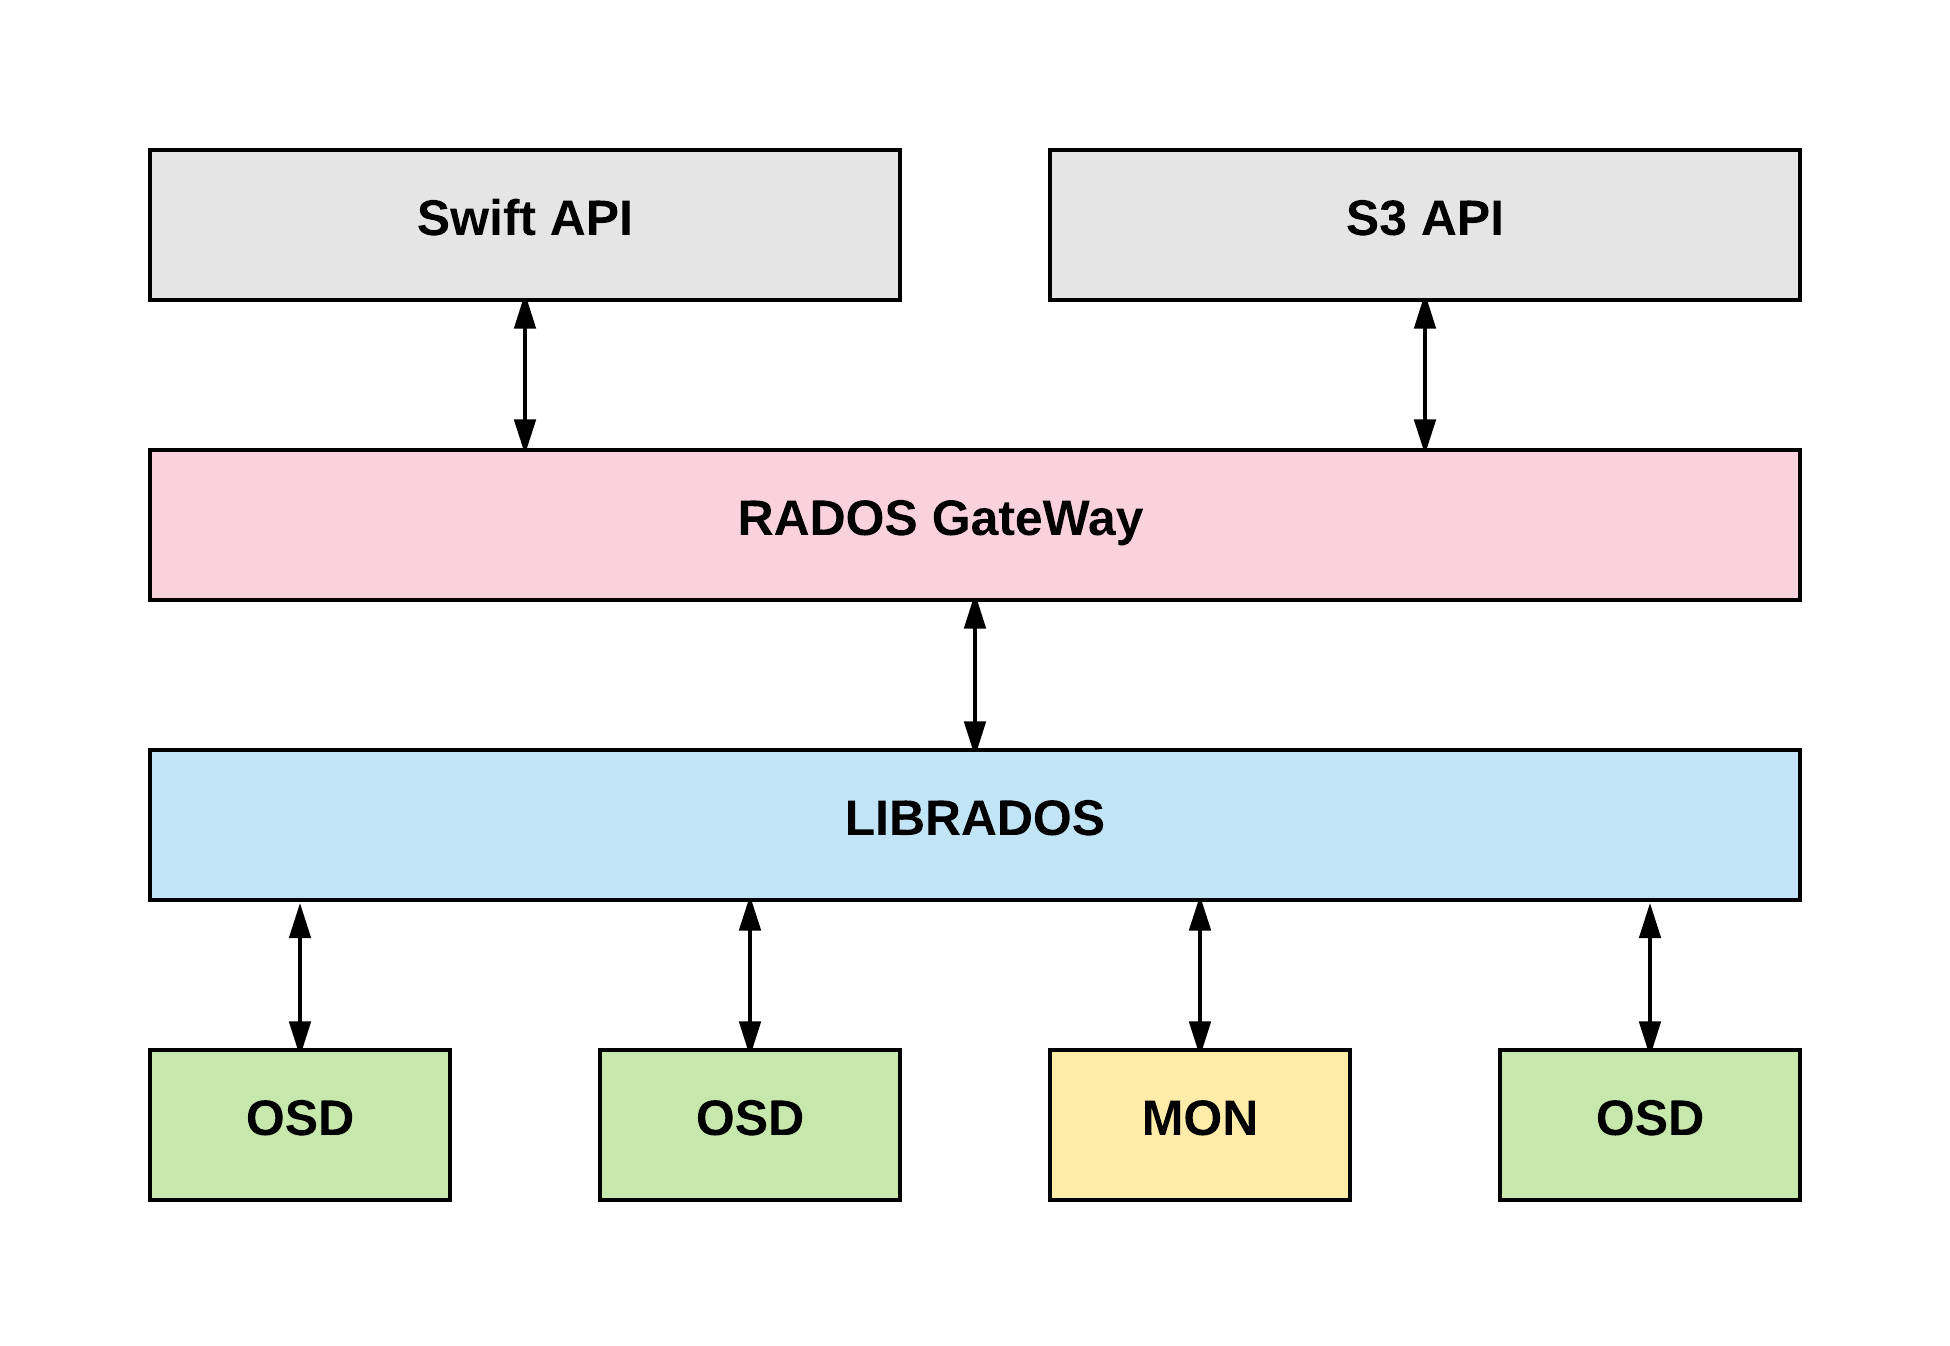
\includegraphics[width=0.65\textwidth]{otherResources/CEPH_RGW_diagram.png} % replace with your diagram
	\end{frame}
		
	\begin{frame}
		\frametitle{Accessing ORFEO}
		\framesubtitle{Centralized identity}
		
		Access to ORFEO is managed through a \textbf{central identity system}:
		
		\begin{itemize}
			\item \textbf{FreeIPA} provides the underlying user and group management.
			\item \textbf{Authentik} builds on top of it to offer modern single sign-on (SSO).
			\item Users log in once and get consistent access across all services.
		\end{itemize}
		
		\vspace{1em}
		\centering
		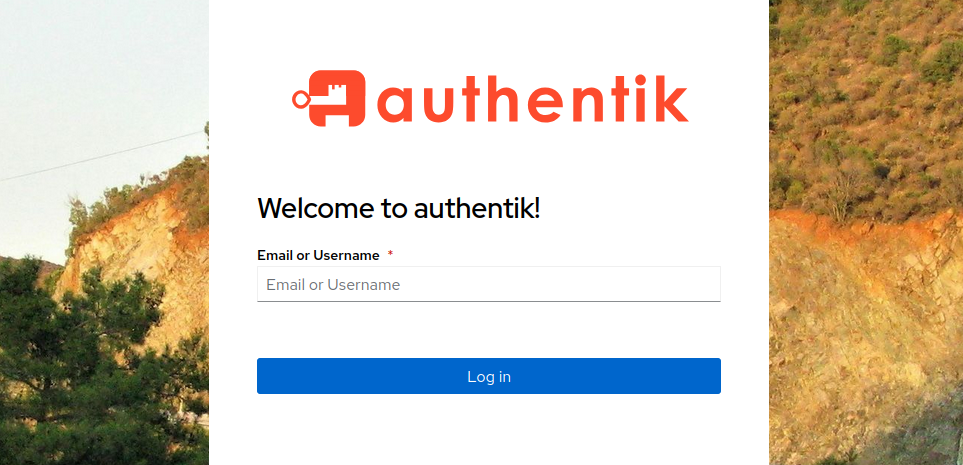
\includegraphics[width=0.65\textwidth]{otherResources/authentik_login.png} % placeholder
	\end{frame}
	
	\begin{frame}
		\frametitle{From problems to a proposal}
		
		\begin{columns}[T,totalwidth=\textwidth]
			\column{0.48\textwidth}
			\textbf{What’s missing for LAME}
			\begin{itemize}
				\item Data often stuck on lab machines or portable drives.
				\item Transfers are manual, with inconsistent folder structures.
				\item No ingestion standard → hard to reuse or integrate with ORFEO/NFFA-DI.
			\end{itemize}
			
			\column{0.48\textwidth}
			\textbf{Our proposal}
			\begin{itemize}
				\item \textbf{Transfer}: move data directly into ORFEO using the S3 protocol.
				\item \textbf{Transform}: convert outputs (e.g.\ TIFF) into NeXus/NXem with standardized metadata.
				\item \textbf{Integrate}: build on ORFEO’s existing services, with a simple web interface and API.
			\end{itemize}
		\end{columns}
	\end{frame}
	
	\begin{frame}
		\frametitle{Choosing a framework}
		
		To put our proposal into practice, we need a tool that researchers can actually use.  
		That means building a \textbf{web application} that can:
		
		\vspace{1em}
		\begin{itemize}
			\item guide researchers through projects, samples, and experiments,
			\item handle uploads and metadata in a consistent way,
			\item connect directly to ORFEO’s services (S3 storage, authentication).
		\end{itemize}
		
		Once this was clear, the next step was to choose the right framework.
	\end{frame}
	
	\begin{frame}
		\frametitle{Why Django?}
		
		We chose Django because it makes it easy to translate lab workflows into software:
		
		\begin{itemize}
			\item \textbf{Models} let us map real-world entities  
			(projects, samples, experiments, measurements) directly into the database.
			\item Comes with both a user-friendly interface and a REST API, so work can be manual or automated.
			\item Plays well with background workers for tasks like checksums and NeXus conversion.
			\item Strong authentication support, fitting smoothly into ORFEO.
		\end{itemize}
	\end{frame}
	
	\begin{frame}
		\frametitle{Thinking about the whole pipeline}
		
		\centering
		\resizebox{\textwidth}{!}{%
			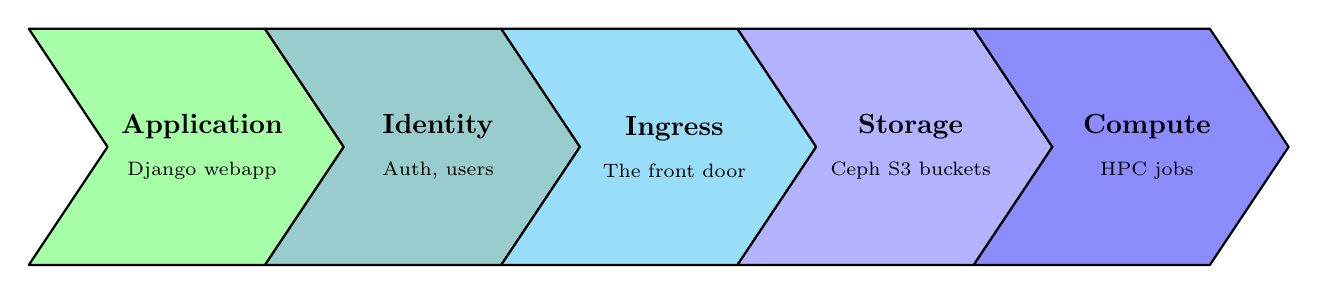
\begin{tikzpicture}[thick]
				
				% geometry
				\def\h{3.0}   % much taller
				\def\w{3.0}   % body width before the tip
				\def\t{1.0}   % tip / notch depth
				
				% one chevron at x-offset #1, with title #2, subtitle #3, and fill color #4
				\newcommand{\chevron}[4]{%
					\begin{scope}[shift={(#1,0)}]
						\path[draw=black, fill=#4, line join=round]
						(0,0) -- (\w,0) -- (\w+\t,0.5*\h) -- (\w,\h) -- (0,\h) -- (\t,0.5*\h) -- cycle;
						% two lines: bold title + smaller subtitle
						\node[align=center, xshift=7mm] at (\w/2,0.5*\h) {\textbf{#2} \\[0.3em] \scriptsize #3};
					\end{scope}
				}
				
				% chain of tall chevrons
				\chevron{0*\w}{Application}{Django webapp}{green!35}
				\chevron{1*\w}{Identity}{Auth, users}{teal!40}
				\chevron{2*\w}{Ingress}{The front door}{cyan!40}
				\chevron{3*\w}{Storage}{Ceph S3 buckets}{blue!30}
				\chevron{4*\w}{Compute}{HPC jobs}{blue!45}
				
			\end{tikzpicture}%
		}
		
		\vspace{1em}
		\small The app is one part of this chain — testing only makes sense when the whole path is reproduced.  
		The solution: a \textbf{digital twin} of ORFEO.
	\end{frame}
	
	% --- 4) VirtualOrfeo ---
	\begin{frame}
		\frametitle{VirtualOrfeo}
		
		ORFEO is a complex infrastructure: identity, ingress, storage, and compute.  
		Testing our Django app directly on production would be risky and slow.
		
		\vspace{1em}
		\begin{itemize}
			\item \textbf{VirtualOrfeo} is a lightweight clone of ORFEO, built on K3s.
			\item It uses the same Helm charts and configs as production.
			\item This lets us deploy the \textbf{Django app} in a realistic environment:
			it can authenticate through Authentik, upload to S3 buckets,
			and be accessed through the same ingress as in ORFEO.
		\end{itemize}
	\end{frame}
	
	\begin{frame}
		\frametitle{VirtualOrfeo topology}
		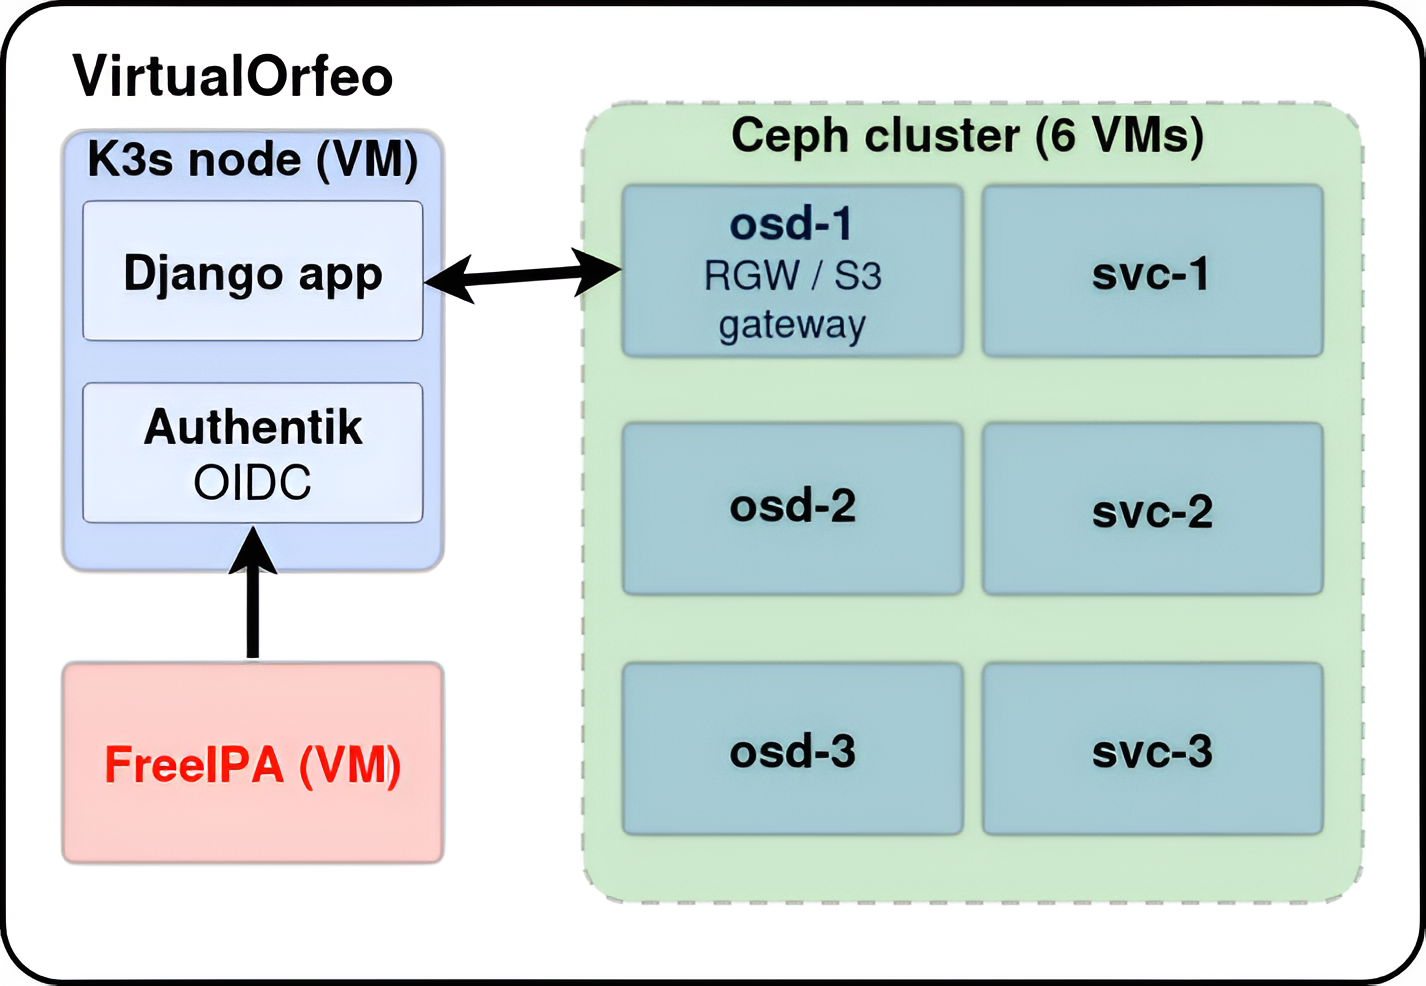
\includegraphics[width=\textwidth]{otherResources/VirtualOrfeo_topology.png}
	\end{frame}
	
	% --- 5) App walkthrough ---	
	\begin{frame}
		\frametitle{Application overview}
		
		The webapp is designed around three main pillars that keep data organized, 
		easy to move, and ready to be reused:
		
		\vspace{0.8em}
		\begin{itemize}
			\item \textbf{Structure} — organize research work into a consistent model.
			\item \textbf{Flow} — move data reliably into storage with linked metadata.
			\item \textbf{Automation} — offload heavy tasks to background workers.
		\end{itemize}
	\end{frame}
	
	% --- Research data model ---
	\begin{frame}
		\frametitle{Research data model}
		
		The app organizes research work in a structured chain:
		
		\vspace{1em}
		\centering
		\resizebox{\textwidth}{!}{%
			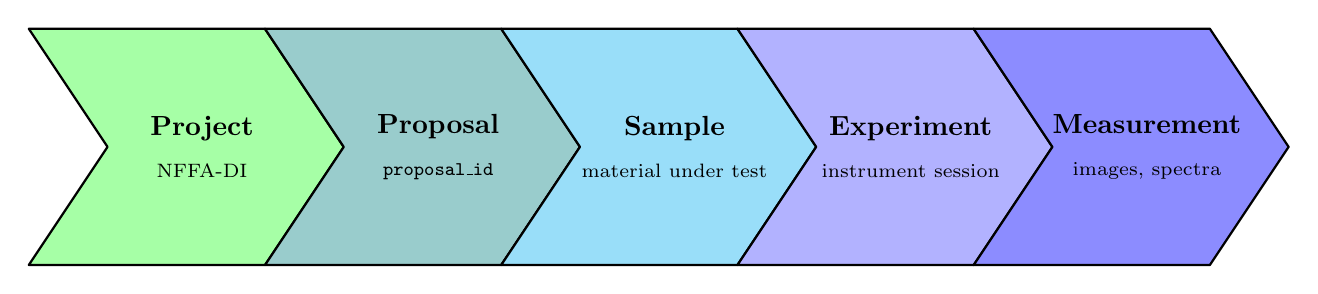
\begin{tikzpicture}[thick]
				
				% geometry
				\def\h{3.0}
				\def\w{3.0}
				\def\t{1.0}
				
				\newcommand{\chevron}[4]{%
					\begin{scope}[shift={(#1,0)}]
						\path[draw=black, fill=#4, line join=round]
						(0,0) -- (\w,0) -- (\w+\t,0.5*\h) -- (\w,\h) -- (0,\h) -- (\t,0.5*\h) -- cycle;
						\node[align=center, xshift=7mm] at (\w/2,0.5*\h)
						{\textbf{#2} \\[0.3em] \scriptsize #3};
					\end{scope}
				}
				
				% chain
				\chevron{0*\w}{Project}{NFFA-DI}{green!35}
				\chevron{1*\w}{Proposal}{\texttt{proposal\_id}}{teal!40}
				\chevron{2*\w}{Sample}{material under test}{cyan!40}
				\chevron{3*\w}{Experiment}{instrument session}{blue!30}
				\chevron{4*\w}{Measurement}{images, spectra}{blue!45}
				
			\end{tikzpicture}%
		}
		
		\vspace{1em}
		\small
		This keeps context together with raw data, making results easier to track and reuse.
	\end{frame}
	
		% --- Managing research data in practice ---
		\begin{frame}
			\frametitle{Managing research data in practice}
			
			\begin{itemize}
				\item Three-pane board to browse and link projects, samples, and experiments.
				\item Metadata (context) stored alongside raw data (\texttt{README.txt}).
				\item Same operations available via REST API for automation.
			\end{itemize}
			
			\vspace{1em}
			\centering
			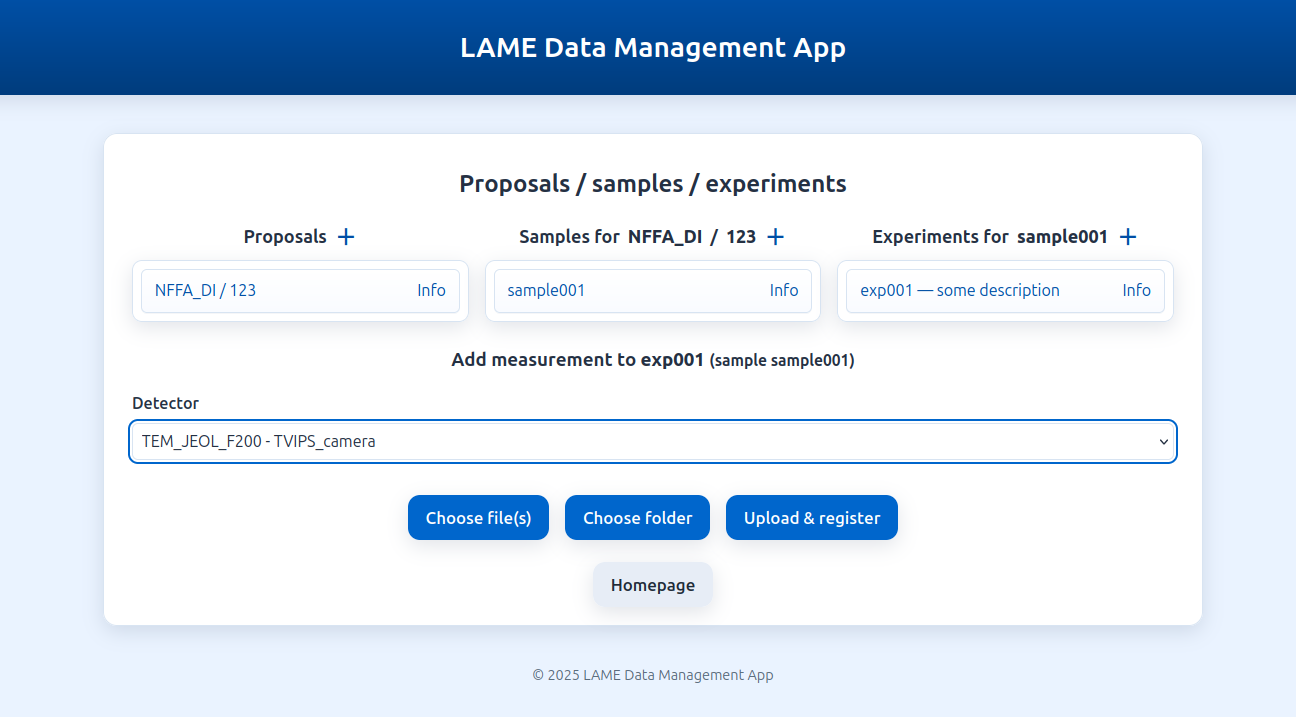
\includegraphics[width=0.8\textwidth]{otherResources/ui_add_measurement.png}
		\end{frame}
	
	% --- Uploading data ---
	\begin{frame}
		\frametitle{From upload to storage}
		
		\begin{itemize}
			\item The app issues a one-time presigned URL.
			\item Browser streams data \textbf{directly to S3}, bypassing the webserver.
			\item Uploads automatically trigger a background job:
			checksum $\to$ metadata extraction $\to$ NeXus build.
		\end{itemize}
		
		\vspace{1em}
		\centering
		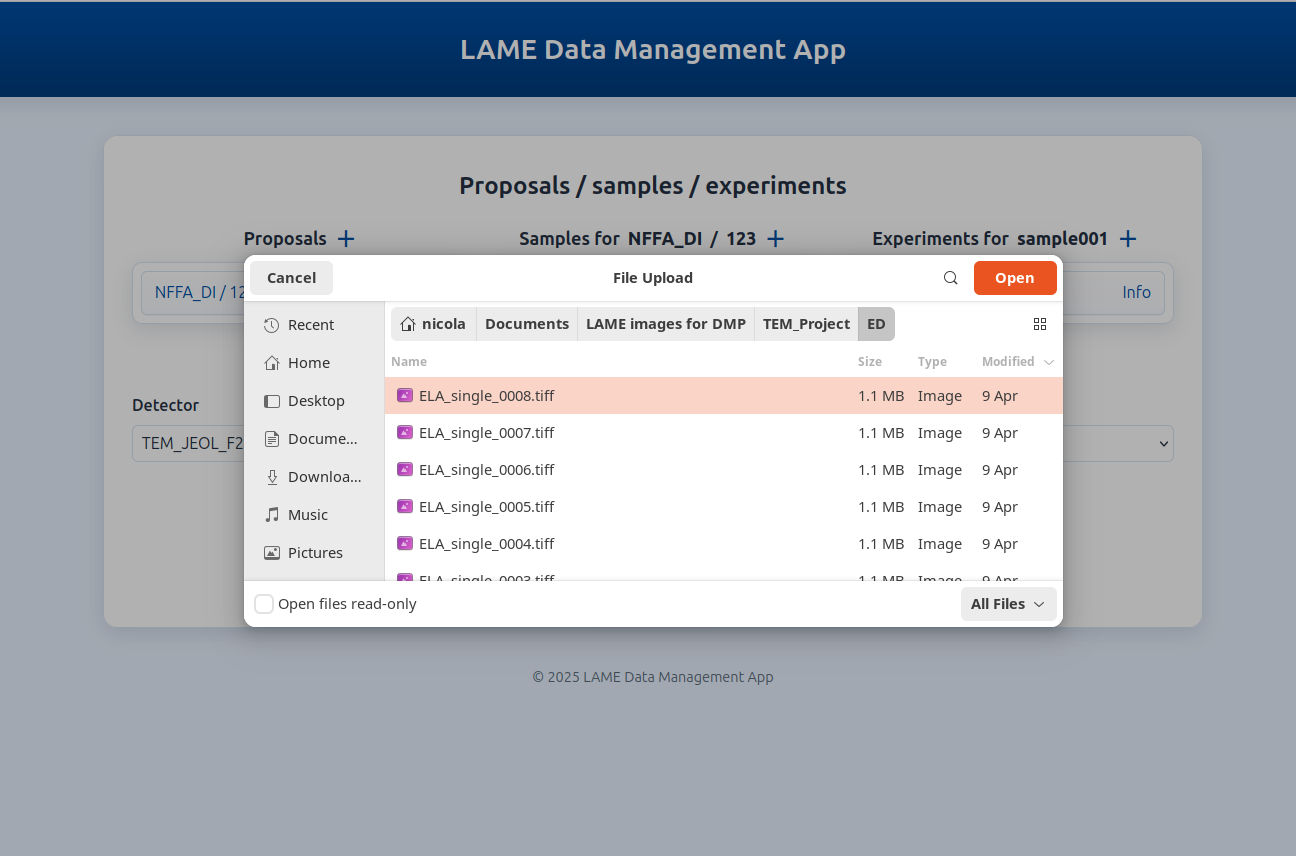
\includegraphics[width=0.6\textwidth]{otherResources/ui_file_picker.png}
	\end{frame}
	
	% --- Workers and NeXus pipeline ---
	\begin{frame}
		\frametitle{Background workers: from raw files to NeXus}
		
		\begin{itemize}
			\item A \textbf{worker pod} runs in the cluster, always listening to Redis (a shared \textbf{to-do list}).  
			\item When a file is uploaded, the app enqueues jobs such as:  
			\begin{itemize}
				\item Metadata extraction (parse TIFF headers or JSON).  
				\item Normalization into NXem fields.  
				\item NeXus generation: structured \texttt{.nxs} file with metadata.  
			\end{itemize}
			\item Jobs are picked up one by one, retried automatically if they fail.  
		\end{itemize}
	\end{frame}
	
	% --- Browsing and sharing ---
	\begin{frame}
		\frametitle{Browsing and sharing data}
		\framesubtitle{Buckets and downloads}
		
		\begin{itemize}
			\item Browse buckets and datasets directly from the interface.
			\item Download with short-lived presigned links.
			\item Create on-the-fly ZIP archives for folders.
			\item Derived data stored in mirrored namespaces for clarity.
		\end{itemize}
		
		\vspace{1em}
		\centering
		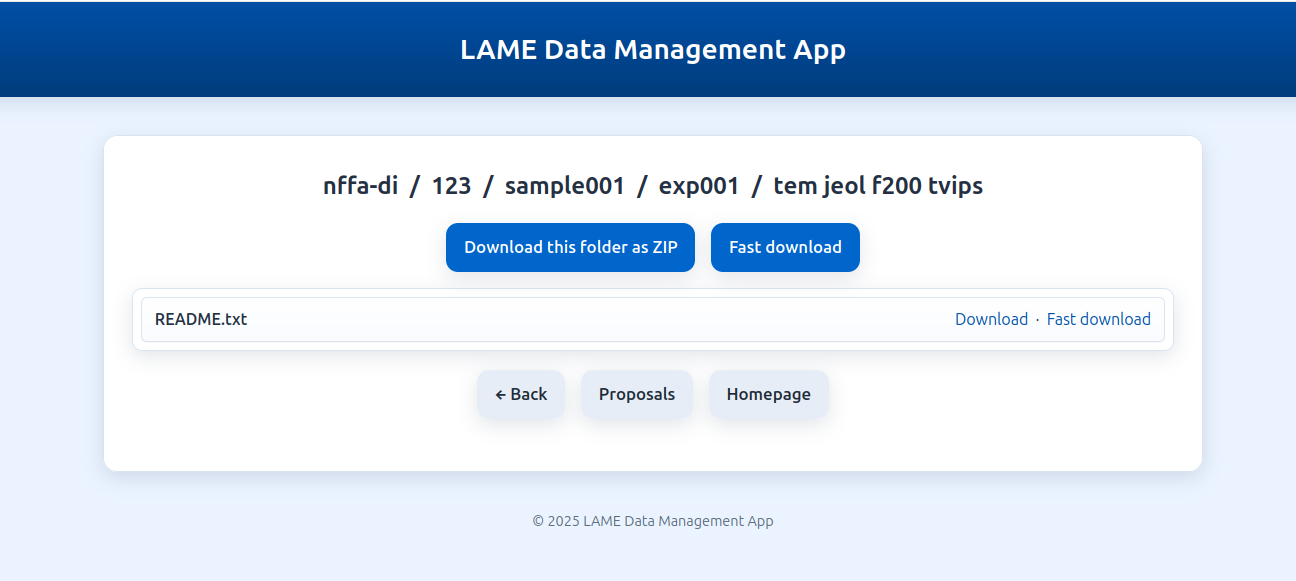
\includegraphics[width=0.8\textwidth]{otherResources/ui_bucket_experiment.png}
	\end{frame}
	
	% --- Live demo ---
	\begin{frame}
		\centering
		\vfill
		{\Huge \textbf{Live Demo}} \\[1.5em]
		{\Large Let’s see the workflow in action.}
		\vfill
	\end{frame}
	
	\begin{frame}
		\centering
		\vfill
		{\Huge \textbf{Thank you for your attention!}} \\[1.5em]
		\vfill
	\end{frame}
	
\end{document}
